%% Copernicus Publications Manuscript Preparation Template for LaTeX Submissions
%% ---------------------------------
%% This template should be used for copernicus.cls
%% The class file and some style files are bundled in the Copernicus Latex Package, which can be downloaded from the different journal webpages.
%% For further assistance please contact Copernicus Publications at: production@copernicus.org
%% https://publications.copernicus.org/for_authors/manuscript_preparation.html

%% copernicus_rticles_template (flag for rticles template detection - do not remove!)

%% Please use the following documentclass and journal abbreviations for discussion papers and final revised papers.

%% 2-column papers and discussion papers
\documentclass[essd, manuscript]{copernicus}



%% Journal abbreviations (please use the same for preprints and final revised papers)

% Advances in Geosciences (adgeo)
% Advances in Radio Science (ars)
% Advances in Science and Research (asr)
% Advances in Statistical Climatology, Meteorology and Oceanography (ascmo)
% Annales Geophysicae (angeo)
% Archives Animal Breeding (aab)
% Atmospheric Chemistry and Physics (acp)
% Atmospheric Measurement Techniques (amt)
% Biogeosciences (bg)
% Climate of the Past (cp)
% DEUQUA Special Publications (deuquasp)
% Drinking Water Engineering and Science (dwes)
% Earth Surface Dynamics (esurf)
% Earth System Dynamics (esd)
% Earth System Science Data (essd)
% E&G Quaternary Science Journal (egqsj)
% EGUsphere (egusphere) | This is only for EGUsphere preprints submitted without relation to an EGU journal.
% European Journal of Mineralogy (ejm)
% Fossil Record (fr)
% Geochronology (gchron)
% Geographica Helvetica (gh)
% Geoscience Communication (gc)
% Geoscientific Instrumentation, Methods and Data Systems (gi)
% Geoscientific Model Development (gmd)
% History of Geo- and Space Sciences (hgss)
% Hydrology and Earth System Sciences (hess)
% Journal of Bone and Joint Infection (jbji)
% Journal of Micropalaeontology (jm)
% Journal of Sensors and Sensor Systems (jsss)
% Magnetic Resonance (mr)
% Mechanical Sciences (ms)
% Natural Hazards and Earth System Sciences (nhess)
% Nonlinear Processes in Geophysics (npg)
% Ocean Science (os)
% Polarforschung - Journal of the German Society for Polar Research (polf)
% Primate Biology (pb)
% Proceedings of the International Association of Hydrological Sciences (piahs)
% Safety of Nuclear Waste Disposal (sand)
% Scientific Drilling (sd)
% SOIL (soil)
% Solid Earth (se)
% The Cryosphere (tc)
% Weather and Climate Dynamics (wcd)
% Web Ecology (we)
% Wind Energy Science (wes)

% Pandoc citation processing

% The "Technical instructions for LaTex" by Copernicus require _not_ to insert any additional packages.
% % % From pandoc table feature
% \usepackage{longtable,booktabs,array}
% % \usepackage{calc} % for calculating minipage widths
% % Correct order of tables after \paragraph or \subparagraph
% \usepackage{etoolbox}
% \makeatletter
% \patchcmd\longtable{\par}{\if@noskipsec\mbox{}\fi\par}{}{}
% \makeatother
% % Allow footnotes in longtable head/foot
% \IfFileExists{footnotehyper.sty}{\usepackage{footnotehyper}}{\usepackage{footnote}}
% \makesavenoteenv{longtable}
% 
% tightlist command for lists without linebreak
\providecommand{\tightlist}{%
  \setlength{\itemsep}{0pt}\setlength{\parskip}{0pt}}


%
\begin{document}


\title{Transition from forest to agriculture in the Brazilian Amazon from 1985 to 2021}


\Author[1, 2]{Hugo}{Tameirão Seixas}
\Author[2]{Hilton}{Luis Ferraz da Silveira}
\Author[2]{Alan}{Falcão}
\Author[2]{Fabiana}{Da Silva Soares}
\Author[1]{Ramon}{Bicudo}


\affil[1]{Center for Environmental Studies and Research, University of Campinas, Rua dos Flamboyants 155, Brazil}
\affil[2]{Embrapa Territorial, Av. Soldado Passarinho 303, Brazil}

\runningtitle{Transition from forest to agriculture in the Brazilian Amazon from 1985 to 2021}

\runningauthor{Seixas et al.}


\correspondence{Hugo\ Tameirão Seixas\ (seixas.hugo@protonmail.com)}



\received{}
\pubdiscuss{} %% only important for two-stage journals
\revised{}
\accepted{}
\published{}

%% These dates will be inserted by Copernicus Publications during the typesetting process.


\firstpage{1}

\maketitle


\begin{abstract}
A new dataset was created by calculating the time necessary for deforested forests to transition to agriculture in the Brazillian Amazon biome. The new data can be useful in interdiciplinary studies about land cover and land use change in brazil, its drivers and implications. A main inovation is that the dataset links the deforestation year with the year of agriculture establishment, which can provide new information about this process.
\end{abstract}


\copyrightstatement{The author's copyright for this publication is transferred to institution/company.}


\introduction[Introduction]

Brazil policies since the 1960s were focused on the expansion of the frontier in the Amazon, specially focused in economic income and land security \citep{Carvalho2002, Mcdonald2003, Banerjee2009}. Such development model led to the construction of thousands of kilometers of roads, and the settlement of large scale livestock farms \citep{Carvalho2002, Banerjee2009}. This period was marked with high rates of deforestation of mature forests \citep{Fearnside2005}. At the same time, cattle and soybean productions started to move to the north direction in the Brazilian territory, in which soybeans cultivation areas followed cattle ranches expansion over the Amazon forest \citep{Simon2005, Barona2010, Arima2011}.
This pattern of extensive livestock occupation after deforestation, followed by the establishment of annual crops is very characteristic in the Amazon biome, and persists nowadays.
This process can take several decades to be accomplished, or even less than one year, in which it may be considered as a direct transition from forest to agriculture.

Land cover transitions are known to cause impacts on different scales.
Deforestation and land use changes can affect hidrological processes in large basins \citep{Arias2018}; reduce the forest resilience to extreme events and other sources of perturbation \citep{Boulton2022}; deforestation and farming practices can reduce convective rainfall and increase surface temperature \citep{Maeda2021}; increase carbon emissions \citep{Gatti2021}; cause important impacts on fauna and flora diversity, soil properties and carbon stocks \citep{Nunes2022}; and even negatively impact public health \citep{Ellwanger2020}.

Data on land use and land cover (LULC) classification are evolving rapidly in the last decade.
Initiatives such as MapBiomas \citep{Souza2020}, launched in 2015, which provides high resolution, annual classifications for the Brazilian territory.
Such type of data are essential to analyse LULC change processes, make causal inferences, and understand what drives and what are the impacts of the transformation of the landscape in Brazil.
In this context, this project aims to characterize and quantify the length of the transitions from forest formations to agriculture in the Amazon.
The availability of this data can be useful to the development of interdisciplinary research involved with LULC changes.

\section{Methods}

\subsection{Transition length calculation}

The estimations of transition from forest to agriculture were performed for the Amazon biome region, as defined by the Brazilian Institute of Geography and Statistics (IBGE), in 2019.
Transitions were calculated using land use and land cover classification data from MapBiomas, which ranges from 1985 to 2021, at a spatial resolution of approximately 30 meters.
The data was filtered to contain only pixels that were occupied by forest and agriculture at some period, and that are not considered as water, according to the Global Surface Water product provided by Copernicus \citep{Pekel2016}.

Transition length was calculated pixel by pixel, by performing the following steps:

\begin{enumerate}
\def\labelenumi{\arabic{enumi}.}
\item
  Load raster and extract valid values into a table;
\item
  Calculate the year of first occurrence of a non-natural LULC class for each pixel;
\item
  Calculate the first year of ``Forest Formation'' LULC class after the year calculated in step 2;
\item
  Classify rows as ``before'' or ``after'' the occurrence of the year calculated in step 3;
\item
  Calculate the last year of ``Forest Formation'' within the rows classified as ``before'', and add 1 year to represent the deforestation year;
\item
  Calculate the first year of any agriculture type class within the rows classified as ``before'', for each pixel;
\item
  Calculate the difference between years from items 5 and 6 to get the LULC transition length in years, for each pixel;
\end{enumerate}

The steps 2 to 7 are performed recursively to identify multiple transitions, in case they are present.
Because of the amount of data, the processing and storage was performed in batches of data, structured in raster tiles.

\subsection{Accuracy assessment}

The accuracy assessment was performed by visual inspection of annual composites of Landsat images from MapBiomas.
We selected 100 random points to be analysed.
An area of approximately 4 squared kilometers around the sample point was used in the visual inspection of satellite images.

The visual inspection used several variables derived from the Landsat historical collection.
The median of Red, Green, Blue, Near Infrared (NIR) and Short Wave Infrared (SWIR1) from dry and wet season were used, and also the annual amplitude of the Normalized Difference Vegetation Index (NDVI).
The process of accuracy assessment was performed in a Shiny app, and was conducted without any consultation to the transition length results.
In the validation app, we estimated, by visual inspection, the year of deforestation and the year of agriculture establishment.
The observed transition length was obtained by subtracting both dates.

To evaluate the accuracy, we calculated the Mean Absolute Error (MAE), the Bias (BIAS), and the Percent Bias (PBIAS).
We also analysed the results by plotting the errors as frequency bars, and scatter plots between observed and estimated values.

After the completion of the analysis of the 100 sample points, we also conducted a qualitative assessment, where we compared our results with the satellite images.

\section{Description of data collection}

After the calculation of transitions, the results are stored in three different types of tables, organized in a folder structure and stored as Apache Parquet files.

\begin{itemize}
\item
  Tables that contains the spatial information (longitude, latitude) of each pixel, its unique id and the code of the municipality which contains the pixel.
  It is named as ``mask\_cells'';
\item
  Tables with transition length values, the first and last year of the transition, the resulting agriculture type, and the number of the transition cycle.
  They also contain the unique id of each pixel (related to the table above);
\item
  Table with the LULC classes of all years within the transition, and also the first 5 years after the transition.
\end{itemize}

The three tables are related to each other and can be used altogether, and are separated by tiles.
Another table containing the metadata of each tile is also created, and holds the spatial characteristics of the tiles.
With this spatial information, it is possible to convert the tabular data back to spatial raster, with identical spatial properties as the MapBiomas classification data.

\section{Results and discussion}

The transition calculations shows that between 1985 and 2021, 64874 squared kilometers of forests were converted to agriculture, in the Brazilian Amazon biome.
The length of the transitions can go from 0 to 35 years, in which transitions closer to 0 year are considered as fast transitions, and transitions closer to 35 years are considered as slow transitions.
Transitions of 0 year are considered as ``direct'' transitions, where there were no presence of pasture before the establishment of agriculture, our estimations shows that around 9.2 \% of the transitions are considered as ``direct''.

Although we named as deforestation the last years identified as forest before classification of antropic cover, we acknowledge that it is not a direct measurement of deforestation (such as PRODES), it is however a proxy to deforestation.

\subsection{Transition patterns}

Transitions from forest to agriculture can be found in almost every region in the Amazon, but is mostly concentrated in clusters, specially in the south and east of the biome, in the states of Mato Grosso, Pará and Maranhão (Figure \ref{fig:map-plot}).

\begin{figure}[ht]
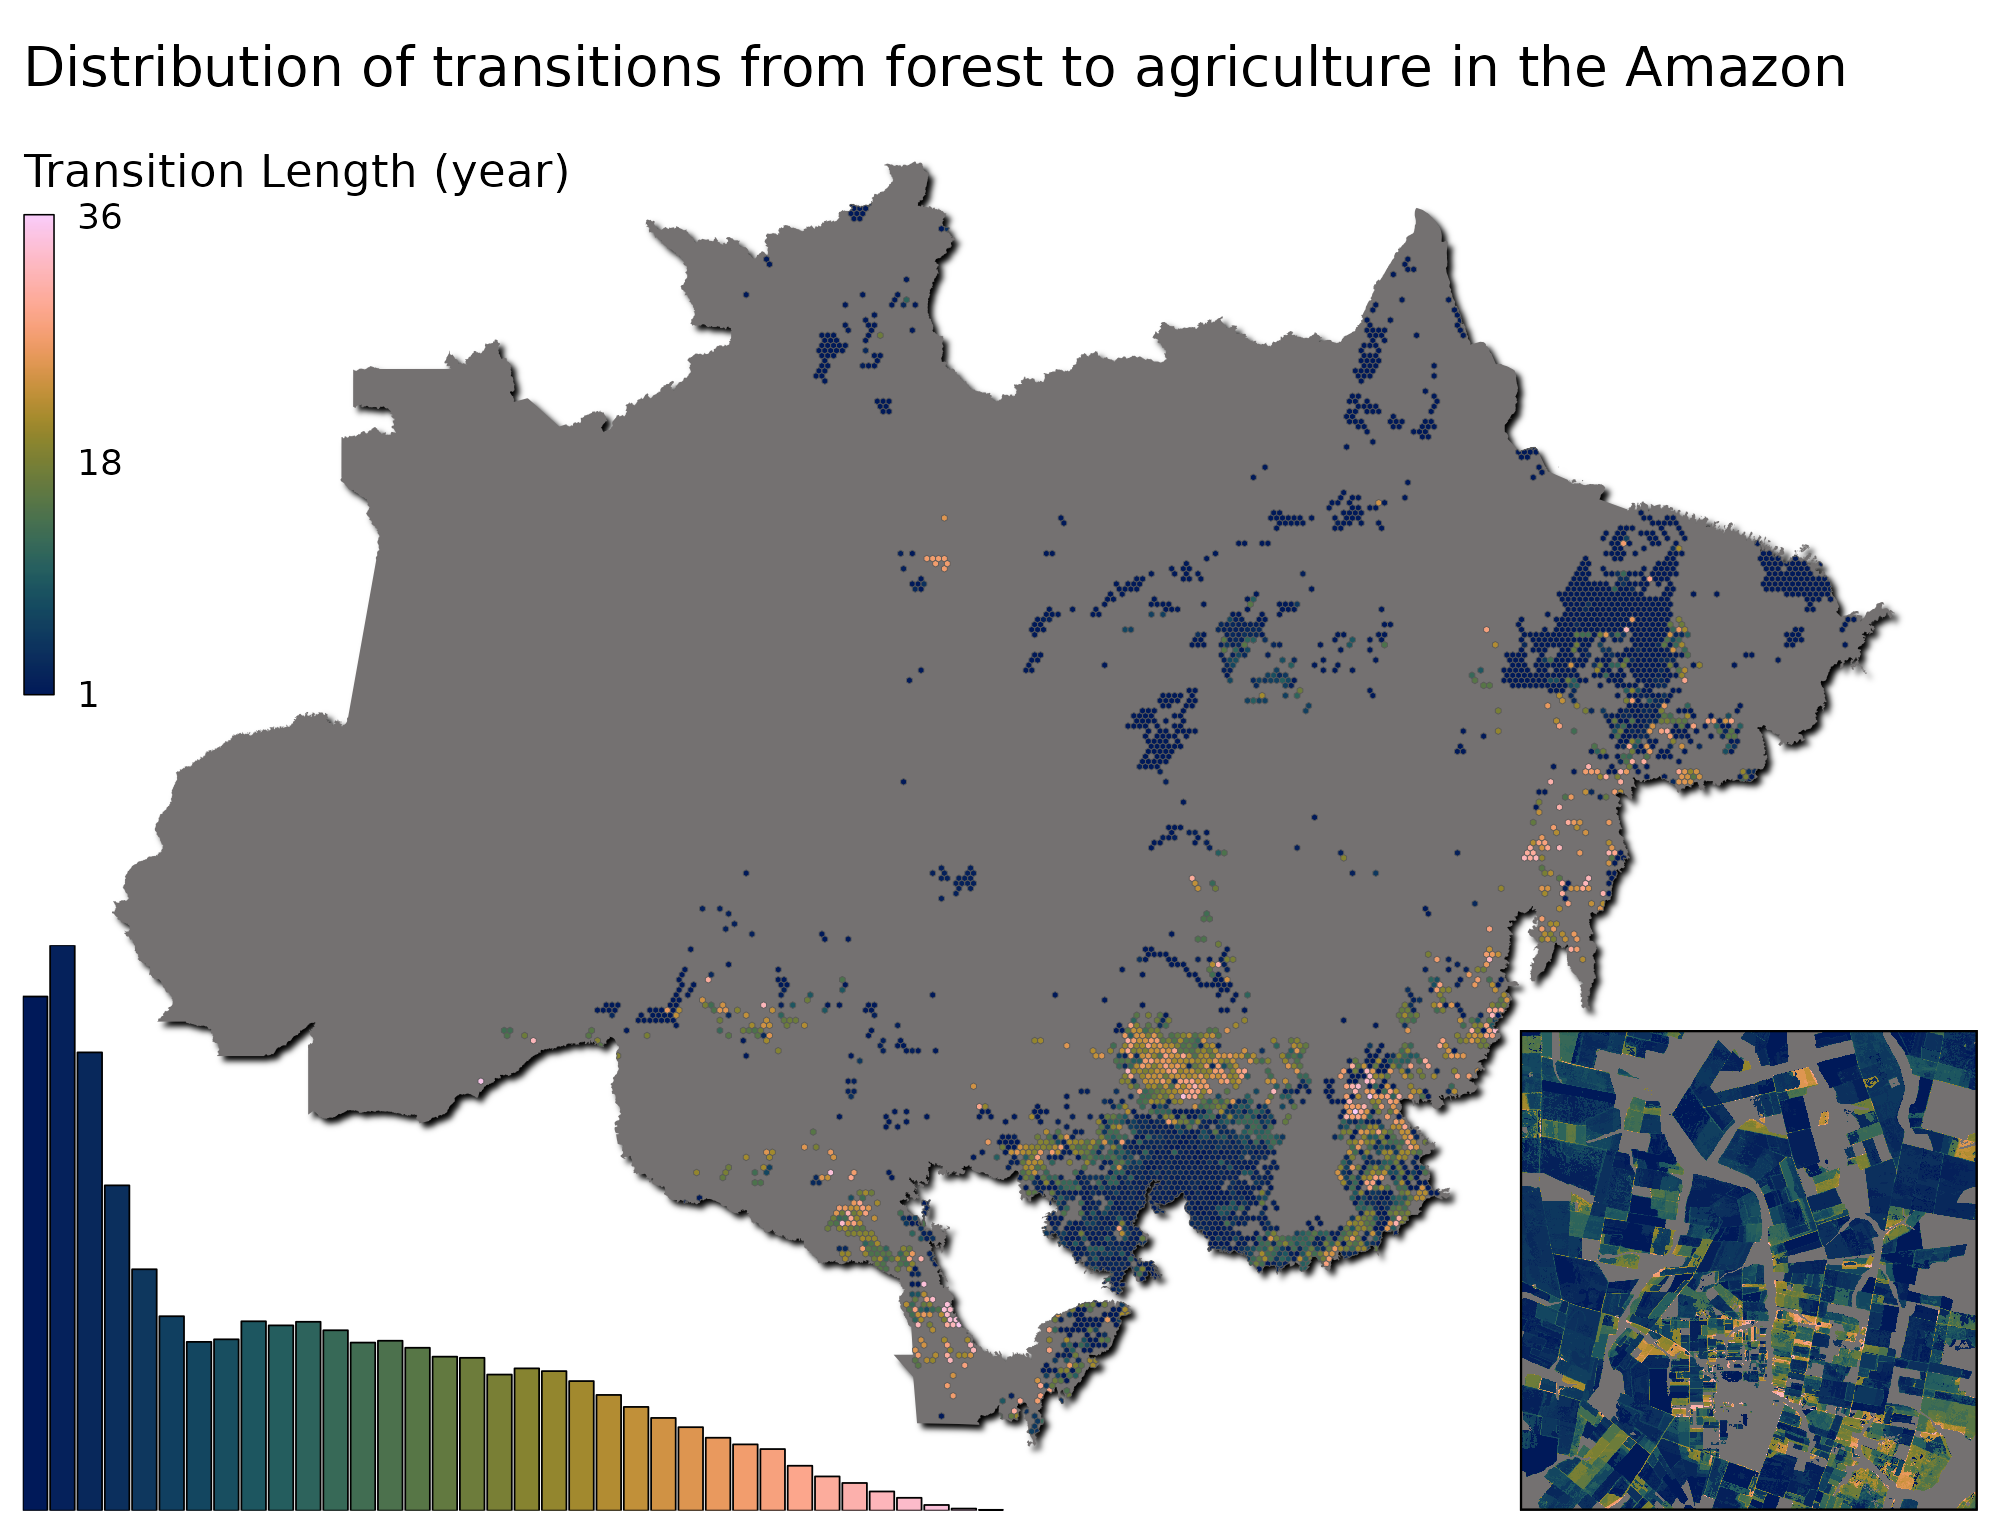
\includegraphics[width=17cm]{figs/map} \caption{Map of distribution of transitions from forests to agriculture in the Brazillian Amazon biome. The hexagonal cells represent the most common transition length, and do not reflect the amount of area of transitions inside a cell. Transitions are concentraded in the south (Mato Grosso state), and in the east (Pará and Maranhão states). The transition length ranges from 1 (blue tones) to 36 years (pink tones), and clusters of fast transitions (transitions closer to 1 year) can be discerned from clusters of slow transitions (transitions closer to 36 years). The histogram located in the bottom left shows that fast transitions are more common than slower transitions. The zoomed map in the bottom right shows the results in finer resolution, where it is possible to observe different transition lengths between properties.}\label{fig:map-plot}
\end{figure}

Well defined clusters can be observed in the map created with aggregated transition length data (Figure \ref{fig:map-plot}), slow transition areas tend to concentrate in specific regions in the Amazon biome, while fast transitions seem to have a wider distributions, but also tend to form clusters.
However, this pattern does not hold completely when observing the data at its original scale (Figure \ref{fig:map-plot}), where areas with different transition lengths are mixed between each other.
When observing at the original scale, we could not spot any well defined pattern or direction of the occurrence of faster to slower transitions (Figure \ref{fig:map-plot}).

Other studies investigating patterns of transitions in the Amazon also found the formation of clusters of patterns, although there is a big heterogeneity at larger scales \citep{MullerHansen2017}.

The data can be analysed year by year, and also be separated by primary and secondary forests being converted to agriculture (Figure \ref{fig:transbar-plot}).

\begin{figure}[ht]
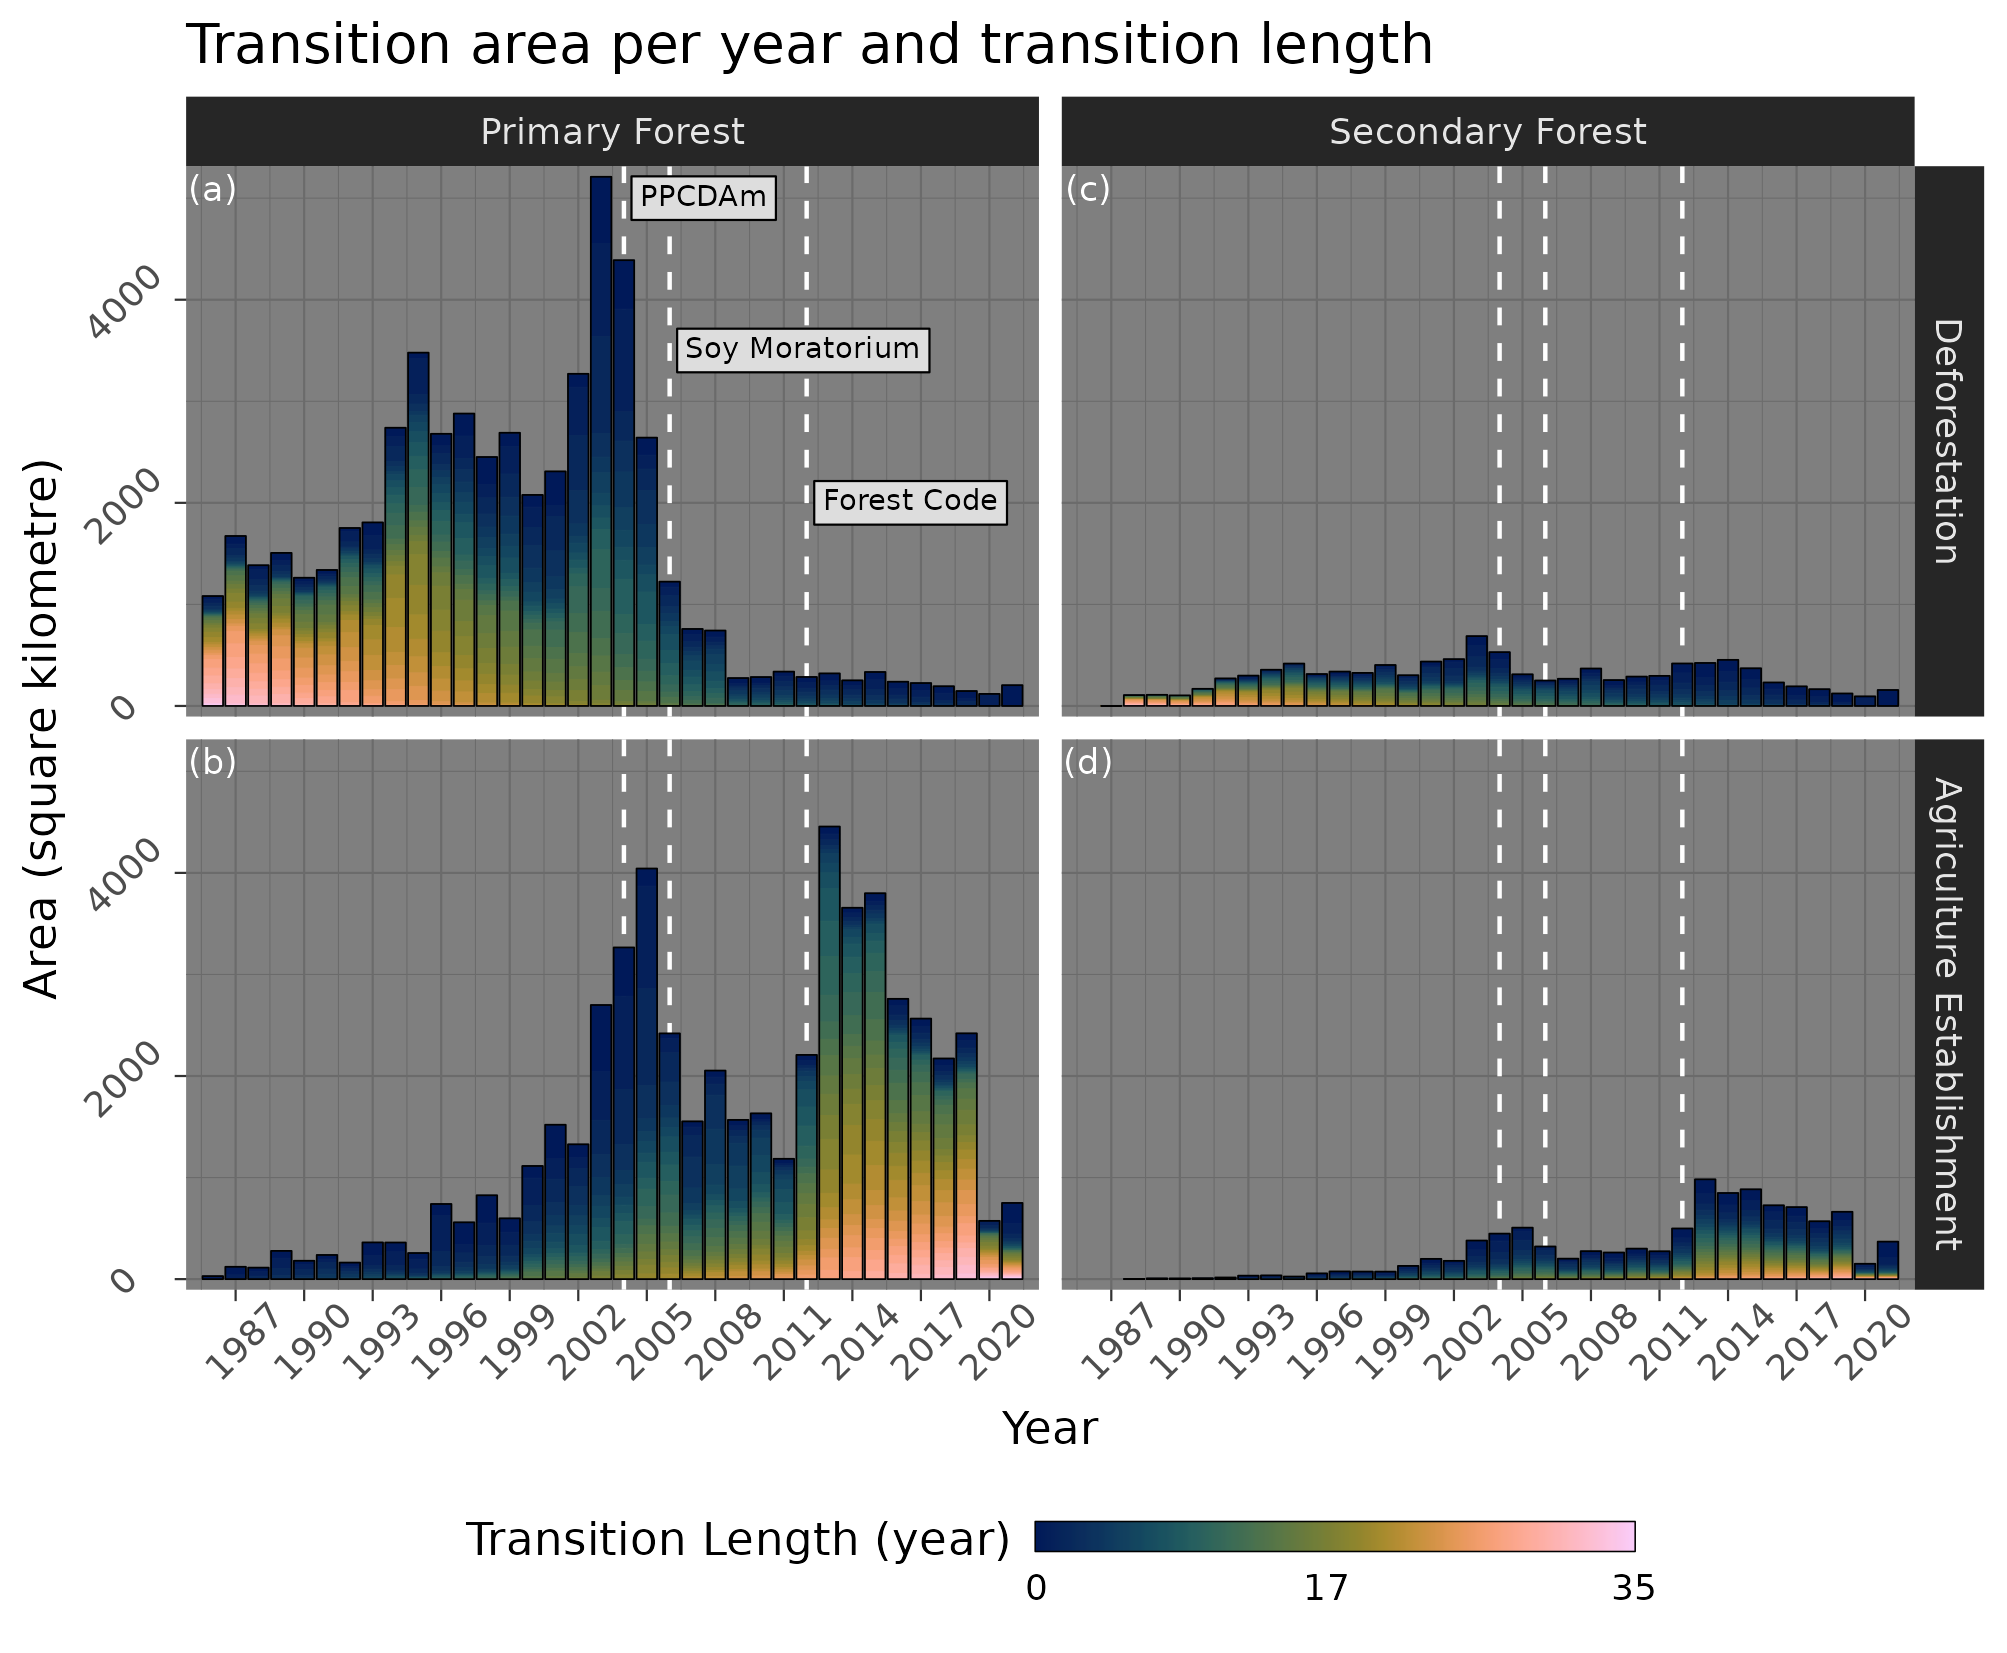
\includegraphics[width=17cm]{figs/trans_length_cols} \caption{Transition area per year and transition length. The bars represent the total amount of area at some state of the transition for each year. The color gradient in each bar represents the transition length related to a deforestation or a agriculture establishment event. Blue tones represents fast transitions (transitions closer to 0 years), pink tones represents slow transitions (transitions closer to 35 years). Transition events were separated by deforestation of primary forests (a) and secondary forests (c), and the subsequent  agriculture establishment of primary forests (b) and secondary forests (d).}\label{fig:transbar-plot}
\end{figure}

TODO: Talk about public policies from 1985 to 2000 (greater carajas program, national environmental policy) \citep{Banerjee2009}.

TODO: Talk about the Avança Brasil plan \citep{Carvalho2002, Banerjee2009}.

TODO: confront our results with Morton 2006 (see the year of 2003).
Confront results from \citep{Macedo2012}, talking about how the expansion of soybean areas are still responsible for production growth, because of very slow transitions.

TODO: talk that even with soy moratorium, and that the deforestation related to transitions were smaller, the deforestation related to pasture occupation kept going, with indirect effects of soybean expansion (Arima 2011).

The deforestation area of primary forests increased largely from 1986 to 2003, which was followed be a steep decrease until 2009, when the deforested areas reached a stable rate.
From 1986 to approximately 1995, most of deforested areas suffered a slow transition, mostly were higher than 10 years, after this period, fast transitions started to become more common, specially from 2002 to 2004.

Agriculture establishment over areas of primary forests peaked in 2005 and 2013.
Despite similar rates between both years, their transition lengths differ greatly, in 2005 most of the transitions were faster than 10 years, while in 2013 the great majority of transitions were slower than 10 years.
The year of 2003 marked a change in the transition length of establishment of agriculture areas, after this year, most of the transitions happened in areas deforested at least 10 years before.
Even after the decrease of deforestation after 2002, agriculture areas are expanding over lands where deforestation happened before 2002.
However, after 2019, a sudden drop of agriculture establishment rate happened.

The causes of deforestation and agriculture establishment in the Brazilian Amazon are complex and diverse.
Political context, public policies, market prices and law enforcement can influence how these processes evolve over time.
In 2004, the Brazilian Government launched the Action Plan for the Prevention and Control of Deforestation in the Legal Amazon (PPCDAm), which was composed by many initiatives to curb deforestation \citep{West2021}.
The PPCDAm was considered as a successful policy to slow deforestation rates in Brazil, with international recognition.
Our calculations from MapBiomas data reinforces the corelation of the PPCDAm with the reduction of deforestation after 2004, and reduction of the agriculture establishment after 2005.

In 2006, the Brazilian Association of Vegetable Oil Industries (BIOVE) and the National Association of Cereal Exporters (ANEC) committed to avoid commercialization of soy grains harvested from areas deforested after 2006.
Our estimates of transitions show a decrease of deforested areas to be converted to agriculture after 2008, where it reached minimal values (Figure \ref{fig:transbar-plot}.a).
After 2006, agriculture establishment over deforested primary forests suffered a decrease, which stayed relatively stable until 2012, where a steep increase occurred, however, the new areas being occupied by agriculture were mainly over areas that were cleared more than a decade before (therefore, before 2006) (Figure \ref{fig:transbar-plot}.b) This shows that agriculture expansion did not halt after the soy moratorium, producers started expanding in old cleared areas.
Expansion of agriculture areas also expanded over cleared areas of secondary forests in 2012, but with an important amount of fast transitions.
The causes of the increase of agriculture establishment areas can be numerous, one main driver was the approval of a new Forest Code, in 2012, which is considered to have undermined the environmental protection of forests \citep{Kroger2017, Pereira2019}.

The transition length patterns across years can change significantly between different states (Figure \ref{fig:transridge-plot}).

\begin{figure}[ht]
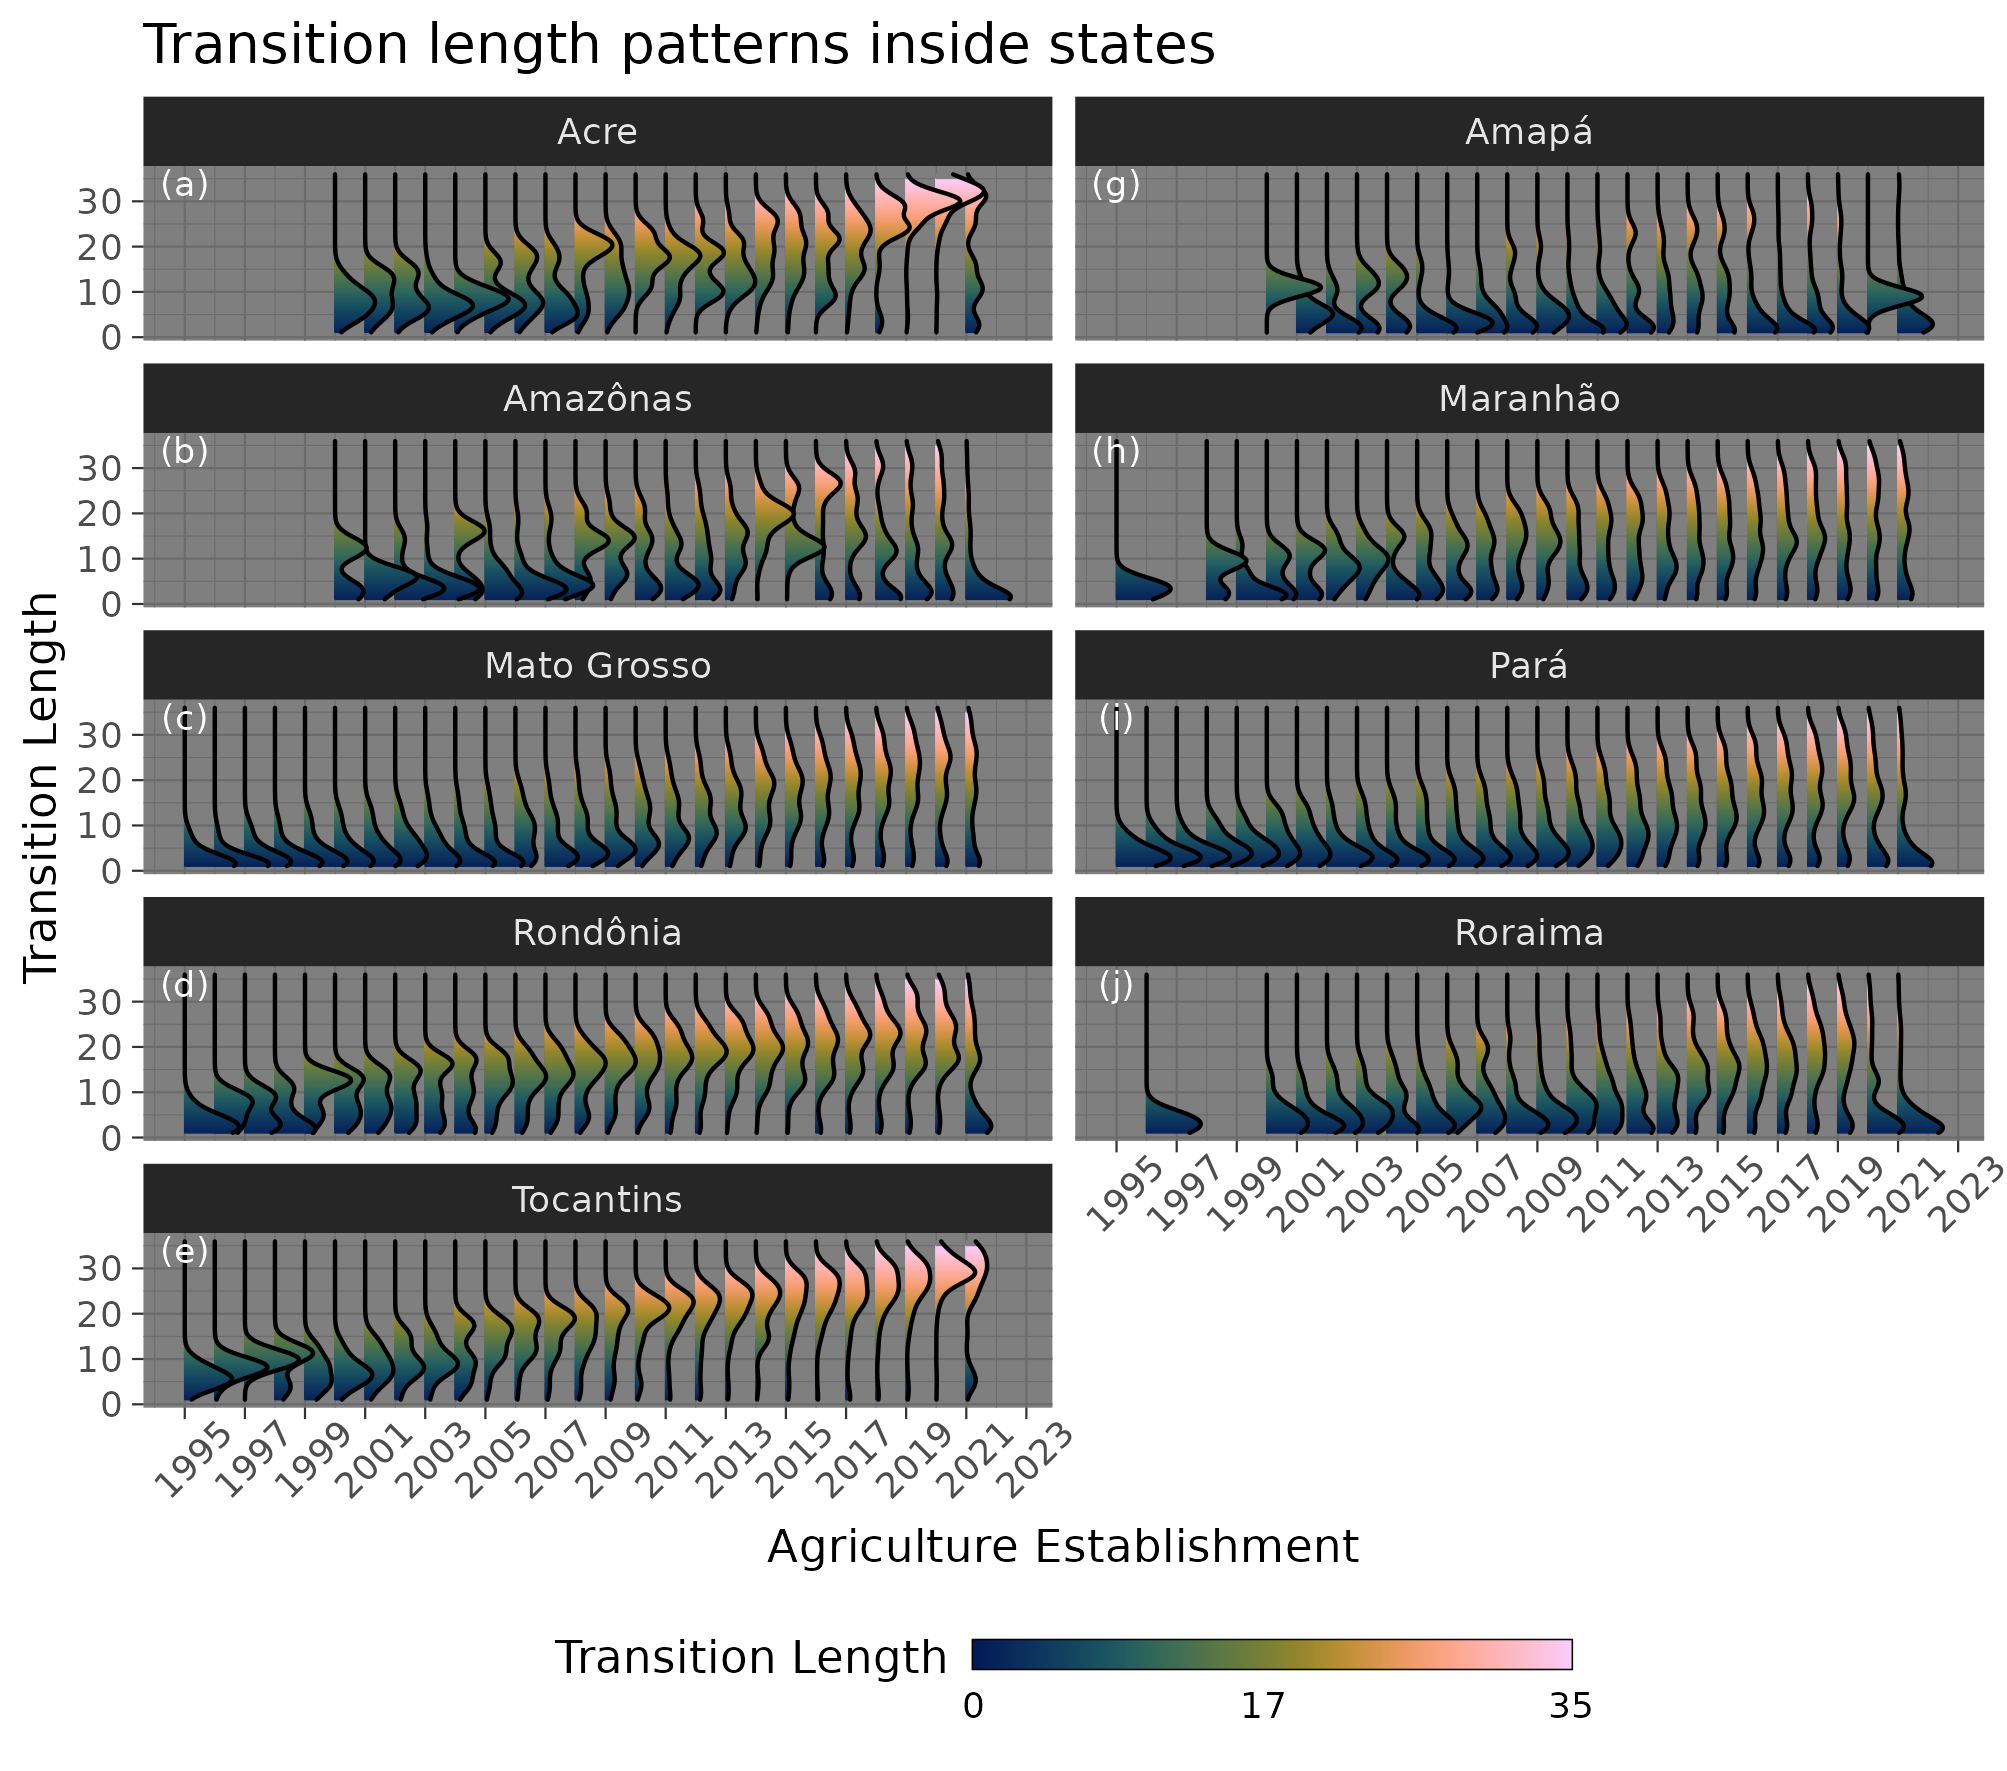
\includegraphics[width=17cm]{figs/trans_ridge} \caption{Transition length patterns inside states that belongs to the Amazon biome. Each year have a density estimate of the transition lengths, represented as colored curves. The peak of the curves represents transition length values with more frequency in one year of one state. Blue tones represents fast transitions (transitions closer to 0 years), pink tones represents slow transitions (transitions closer to 35 years)}\label{fig:transridge-plot}
\end{figure}

The state of Amapá presented fast transitions along all the time series, where slow transitions are not as common.
In contrast, Acre shows a majority of slow transitions, in which only 2021 showed more fast transitions.
There are three states where the pattern of transitions length across time are alike, Mato Grosso and Pará presented more fast transitions from 1995 to 2005, after this period, slow transitions became more common with time.
Rondônia and Tocantins also presented a pattern in which transitions became slower with time, however this pattern started to occur earlier than Mato Grosso and Pará.

The great majority of transitions are from forests to Soybeans and ``Other Temporary Crops'', which represents 95\% of the transitions in the Amazon biome (14\% of Soybean and 81\% of ``Other Temporary Crops'').
When analyzing what happened after 5 years since the transition, Soybean farms are persistent, 79\% of these areas remained as Soybean, 14\% is converted to ``Other Temporary Crops'' and 7\% in occupied by Pasture.
``Other Temporary Crops'' are less persistent, 27\% of these areas remains as the same use, 56\% is converted to Soybean, and 15\% to Pasture.
Conversions from Soybean and ``Other Temporary Uses'' to other covers and uses (apart from the already cited) are negligible.
Sugar Cane, Cotton and Perennial Crops also appears, but in a negligible proportions.

\subsection{Validation}

From the 100 random sample points used in the results validation, 1 point (sample 21) was not considered as a transition from our estimations, however, the visual inspection pointed to a likely event of transition from forest to agriculture.
Also, there were 6 points (sample 6, 7, 55, 56, 78, 97) which the visual inspection did not found a transition from forest to pasture, although our estimations pointed as transitions.
Therefore, 7\% of the sample were completely misclassified by our estimates, and the rest of the accuracy assessment was performed over the remaining 93 sample points.

When analyzing the errors from the transition length estimates, we observe that the year of deforestation shows the least amount of errors (Figure \ref{fig:errorbar-plot}).
The MAE of the deforestation year is of 1.42 years, and the error shows a bias towards underestimation.
The year of the agriculture establishment and the transition length estimates showed larger errors when comparing with visual inspection.

\begin{figure}[ht]
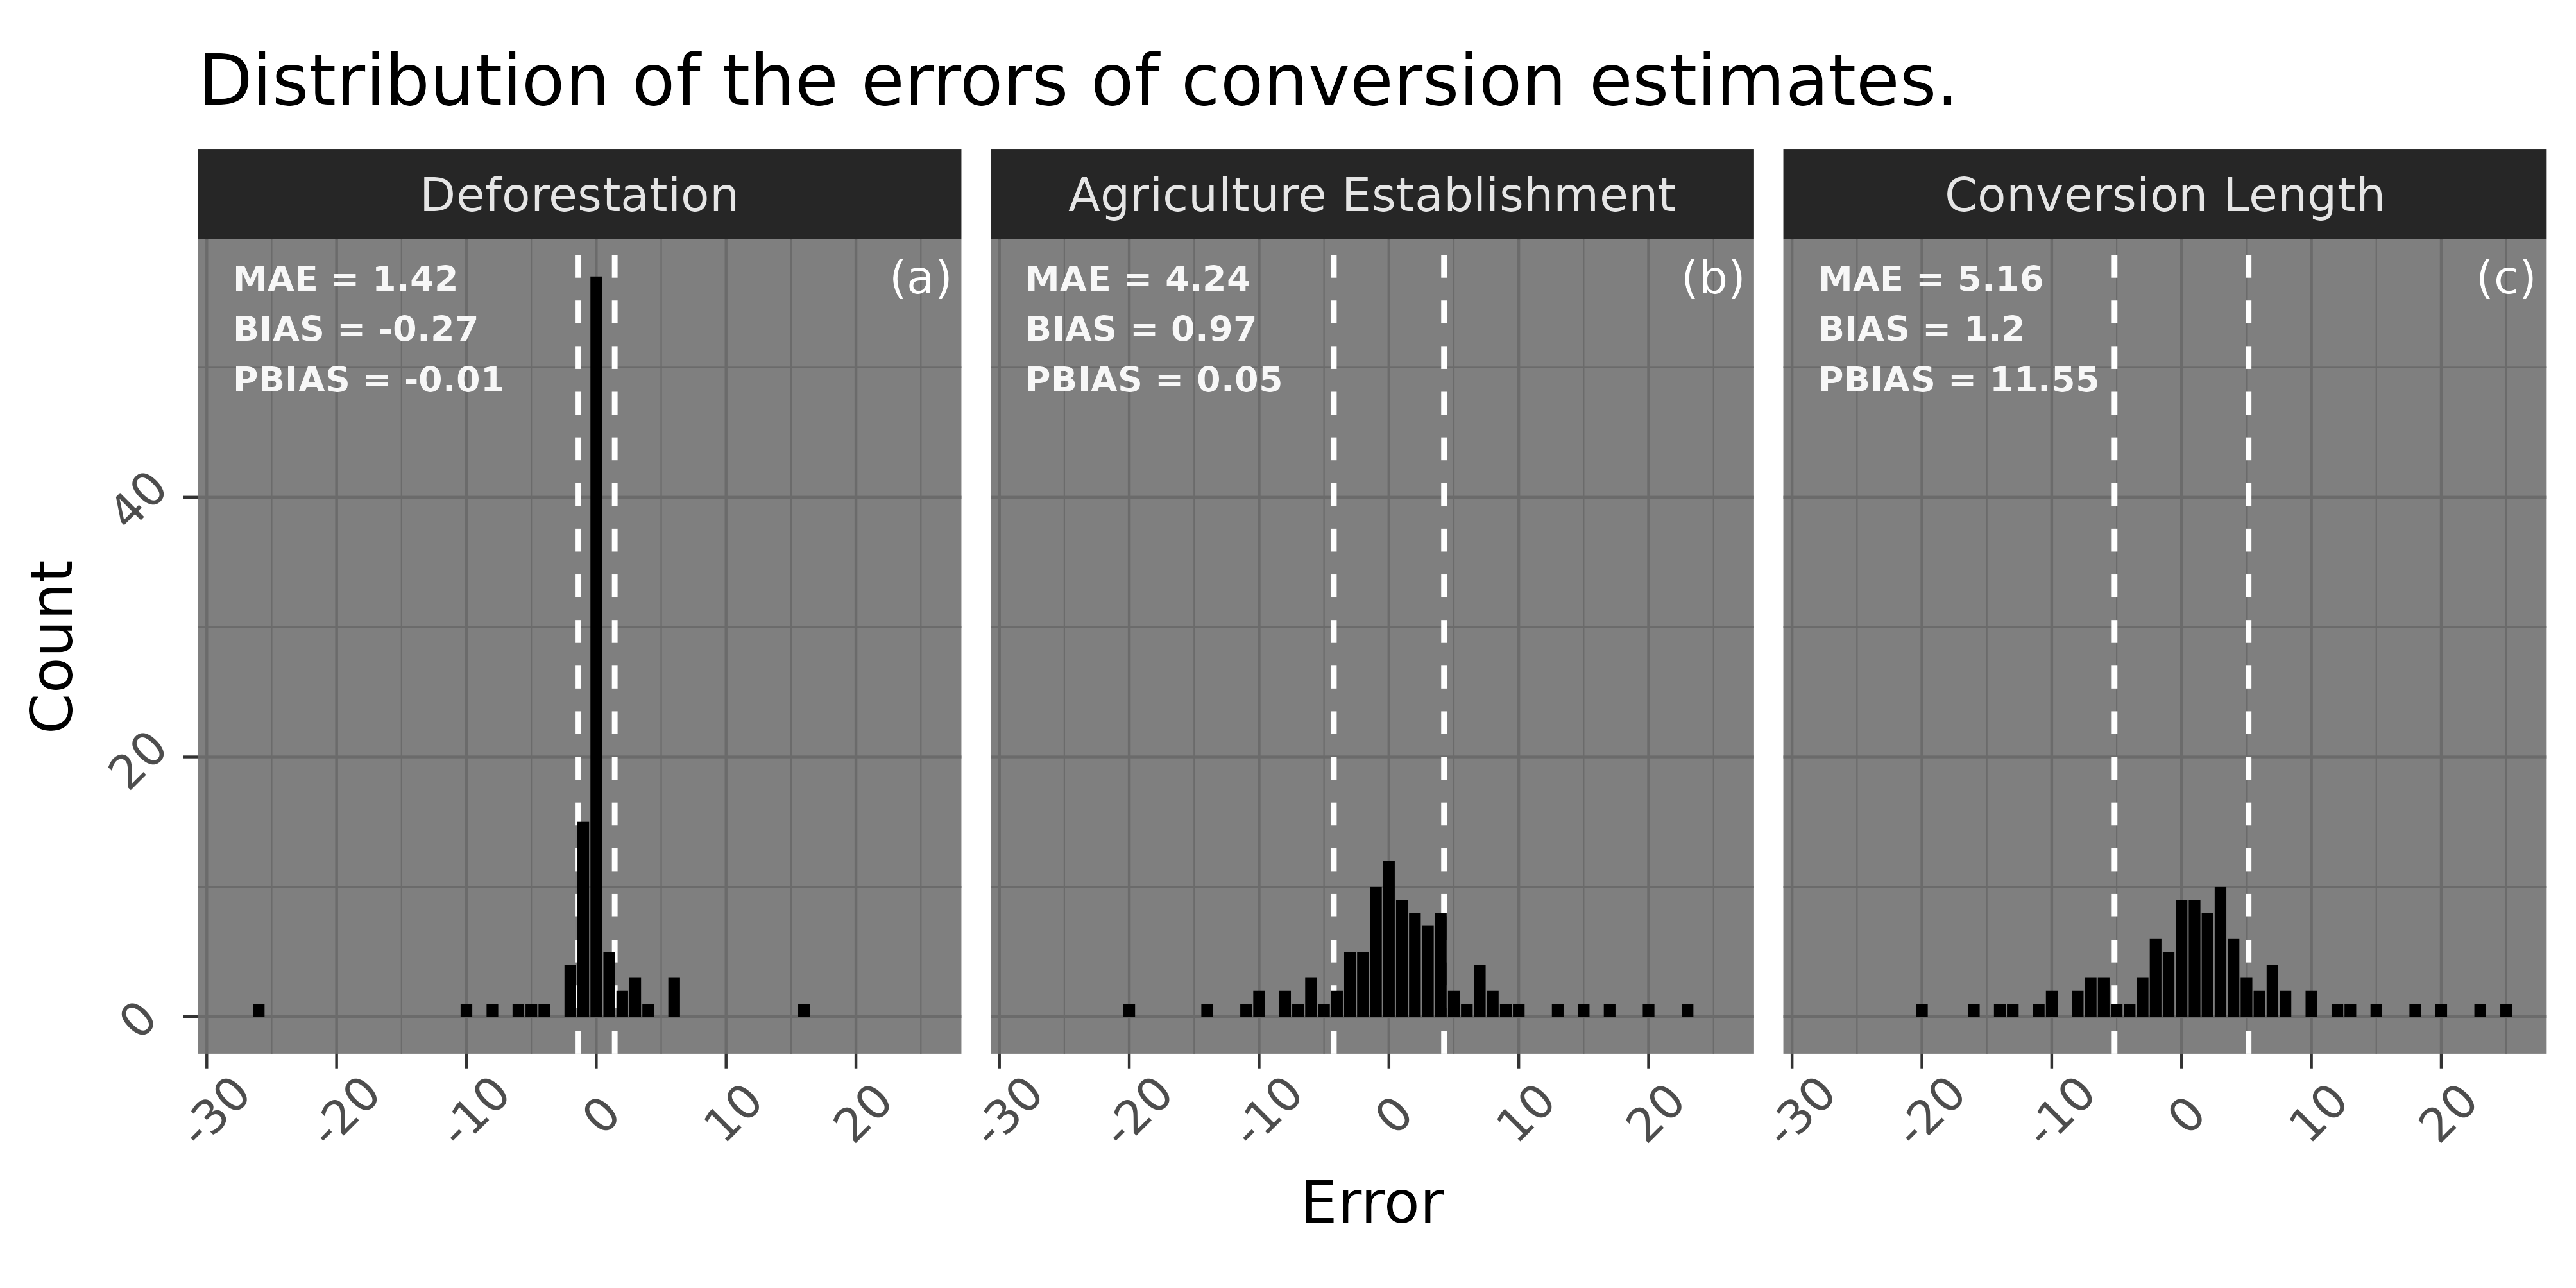
\includegraphics[width=17cm]{figs/error_bars} \caption{Bar with the count of error values (difference between observed and estimated values). Positive values indicate underestimation of the variable (estimations were lower than observations), negative values indicates overestimation (estimations higher than observations). Error metrics (Mean Absolute Error, Bias and Percent Bias) are displayed in the top right position of each box. The white deshed lines represents the MAE values of each variable.}\label{fig:errorbar-plot}
\end{figure}

The dispersion of observed and estimated values shows no clear pattern of errors (Figure \ref{fig:errorscatter-plot}).
Transition length values are more concentrated in smaller values, which also shows higher errors (Figure \ref{fig:errorscatter-plot}.c).
However, this is expected since faster transitions are more common (Figure \ref{fig:map-plot}).

\begin{figure}[ht]
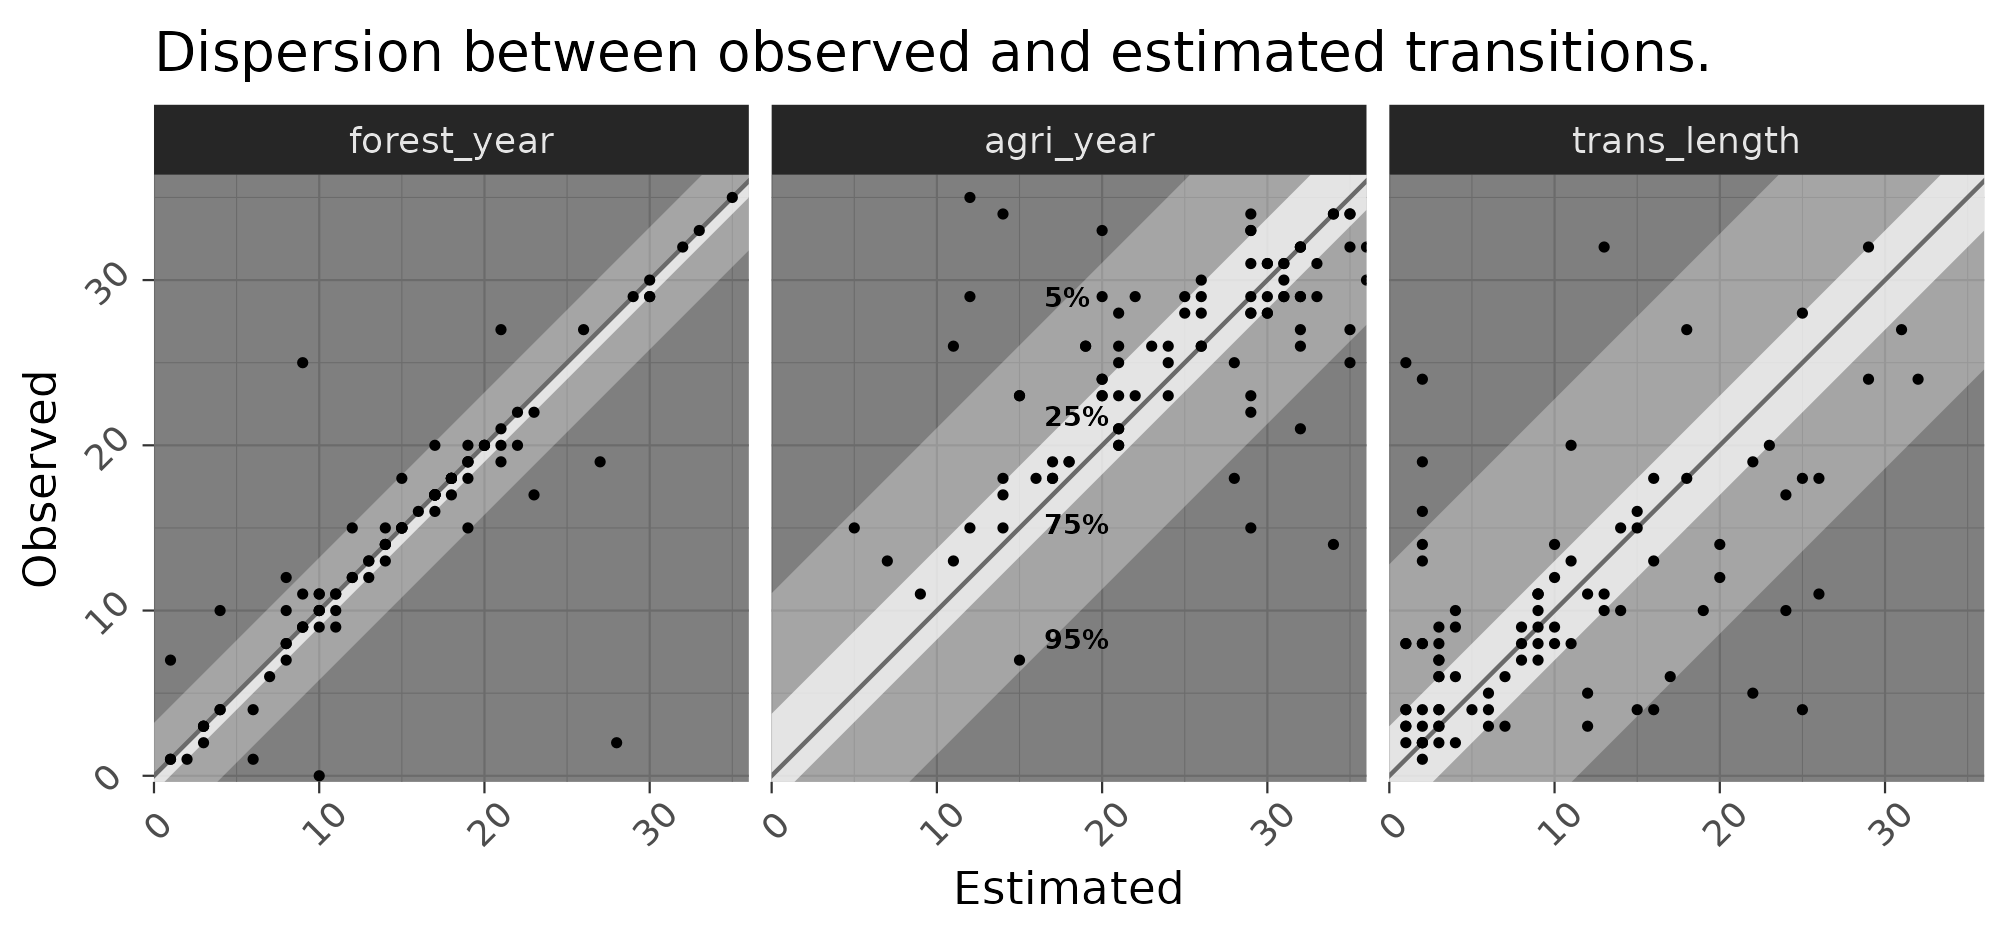
\includegraphics[width=17cm]{figs/error_scatter} \caption{Scatter plot between paired values of estimated and observed Deforestation and Agriculture Establishment years, and their respective Transition Length. Translucid white areas represent quantile ranges (5\%, 25\%, 75\% and 95\%) of the errors. The area between 5\% and 95\% quantiles includes 90\% of points. The area between 25\% and 75\% quantiles includes 50\% of points.}\label{fig:errorscatter-plot}
\end{figure}

According to accuracy assessment from MapBiomas, the collection 7 presents a global accuracy of 96.6\% for the Amazon biome, which is the proportion of pixels that were classified correctly.
For the Forest class, MapBiomas showed small errors of inclusion (proportion of pixels misclassified as other classes, but the real class were Forest), which fluctuated around 1\%.
The omission errors for Forests are also small (proportion of pixels misclassified as Forests, but the real class were not Forest), which fluctuated around 2\%.
The Agriculture class presented more errors, the inclusion errors ranged from 22\% to 5\%, and were mostly composed by Forests pixels (forest pixels misclassified as agriculture).
The omission errors of Agriculture ranged from 22\% to 8\%, and were also mostly composed by Forests pixels (agriculture pixels misclassified as Agriculture).

\subsection{Qualitative assessment}

High heterogeneity inside agriculture plots (sample 56), caused by both year of deforestation or year of agriculture establishment.
Roads being considered as agriculture (sample 2).
Omissions were detected, specially agriculture plots not being considered as a transition as a whole, parts of a plot that were clearly a transition were not considered as a transition (sample 16, 30, 75).
Inclusions were detected, areas that clearly showed no agriculture were considered as transitions (sample 10, 98).
Effect of border on results (sample 25, 56, 84, 92).
Areas with sparse forest vegetation presented large error of deforestation year (sample 33).

Patterns of agriculture areas are roughly well represented (sample 25, 43, 56, 84).
Some locations presents a better homogeneity of transitions inside agriculture plots (sample 84).

Interference due to atmospheric conditions and lack of image availability clearly shaped spatial patterns of transitions at some locations.
Quality of composites trough the time series affected accuracy of results.
Regions of the North part of the Amazon presents lower quality than regions in the South of the Amazon biome.

\conclusions[Conclusions]






%%%%%%%%%%%%%%%%%%%%%%%%%%%%%%%%%%%%%%%%%%
%% optional

%%%%%%%%%%%%%%%%%%%%%%%%%%%%%%%%%%%%%%%%%%

%%%%%%%%%%%%%%%%%%%%%%%%%%%%%%%%%%%%%%%%%%

%%%%%%%%%%%%%%%%%%%%%%%%%%%%%%%%%%%%%%%%%%
\competinginterests{The authors declare no competing interests.} %% this section is mandatory even if you declare that no competing interests are present

%%%%%%%%%%%%%%%%%%%%%%%%%%%%%%%%%%%%%%%%%%

%%%%%%%%%%%%%%%%%%%%%%%%%%%%%%%%%%%%%%%%%%

%% REFERENCES
%% DN: pre-configured to BibTeX for rticles

%% The reference list is compiled as follows:
%%
%% \begin{thebibliography}{}
%%
%% \bibitem[AUTHOR(YEAR)]{LABEL1}
%% REFERENCE 1
%%
%% \bibitem[AUTHOR(YEAR)]{LABEL2}
%% REFERENCE 2
%%
%% \end{thebibliography}

%% Since the Copernicus LaTeX package includes the BibTeX style file copernicus.bst,
%% authors experienced with BibTeX only have to include the following two lines:
%%
\bibliographystyle{copernicus}
\bibliography{references.bib}
%%
%% URLs and DOIs can be entered in your BibTeX file as:
%%
%% URL = {http://www.xyz.org/~jones/idx_g.htm}
%% DOI = {10.5194/xyz}


%% LITERATURE CITATIONS
%%
%% command                        & example result
%% \citet{jones90}|               & Jones et al. (1990)
%% \citep{jones90}|               & (Jones et al., 1990)
%% \citep{jones90,jones93}|       & (Jones et al., 1990, 1993)
%% \citep[p.~32]{jones90}|        & (Jones et al., 1990, p.~32)
%% \citep[e.g.,][]{jones90}|      & (e.g., Jones et al., 1990)
%% \citep[e.g.,][p.~32]{jones90}| & (e.g., Jones et al., 1990, p.~32)
%% \citeauthor{jones90}|          & Jones et al.
%% \citeyear{jones90}|            & 1990


\end{document}
